% !TEX root=../dummy/dummy-02.tex

\section{第 \ref{sec.2.title} 章补充内容}

\subsection{Minnesota 部分子集与 GMTKN55 数据集详细测评表}

\begin{table}[!h]
\centering
\caption[MR-MGM-BE4 子集测评误差]{部分 xDH@B3LYP 模型与 XYG6+1 模型近似泛函在 MR-MGM-BE4 子集上误差。\\反应能与 MUEPB 单位 \si{kcal.mol^{-1}};HOMO/LUMO gap 单位 eV。}
\label{tab.2.supp.MR-MGM-BE4}
\widetabular{
  \begin{tabular}{ld{1.2}d{3.2}d{3.2}d{3.2}d{3.2}d{3.2}d{3.2}}
  \toprule
  \multicolumn{2}{c}{MR-MGM-BE4} & \multicolumn{3}{c}{xDH@B3LYP} & \multicolumn{3}{c}{XYG6+1\tnote{a}} \\
  \cmidrule(lr){1-2} \cmidrule(lr){3-5} \cmidrule(lr){6-8}
  体系 & \multicolumn{1}{c}{gap} & 
  \multicolumn{1}{c}{XYG3} & \multicolumn{1}{c}{XYG6} & \multicolumn{1}{c}{XYG7} &
  \multicolumn{1}{c}{MP2/cr} & \multicolumn{1}{c}{sIEPA} & \multicolumn{1}{c}{IEPA} \\
  \midrule
  \ce{CaO } & 2.54 & 7.01  & 8.03  & 1.50  & 1.41      & 0.18         & 0.68        \\
  \ce{KO- } & 1.03 & 38.03 & 56.57 & 46.24 & 0.00      & 0.00         & 0.00        \\
  \ce{LiO-} & 1.03 & 19.40 & 25.28 & 20.65 & 5.80      & 9.54         & 3.99        \\
  \ce{MgS } & 1.75 & -3.27 & -1.52 & -2.83 & -5.75     & -4.77        & -5.81       \\
  \midrule
  MUEPB     &      & 16.93 & 22.85 & 17.81 & 3.24      & 3.62         & 2.62        \\
  \bottomrule
  \end{tabular}
}{
  \item[a] 为方便排版,表头第二行指代的是 XYG6+1 模型泛函所使用的 EP 型相关能 $E_\textmt{c}^\textmt{EP}$ 的具体类型;即 MP2/cr 指代 XYG6+1/cr、sIEPA 指代 XYG6+1/sIEPA、IEPA 指代 XYG6+1/IEPA。后续表格类同。
}
\end{table}

\begin{table}[!h]
\centering
\caption[SR-MGM-BE9 子集测评误差]{部分 xDH@B3LYP 模型与 XYG6+1 模型近似泛函在 SR-MGM-BE9 子集上误差。\\反应能与 MUEPB 单位 \si{kcal.mol^{-1}};HOMO/LUMO gap 单位 eV。}
\label{tab.2.supp.SR-MGM-BE9}
\widetabular{
  \begin{tabular}{ld{1.2}d{3.2}d{3.2}d{3.2}d{3.2}d{3.2}d{3.2}}
  \toprule
  \multicolumn{2}{c}{SR-MGM-BE9} & \multicolumn{3}{c}{xDH@B3LYP} & \multicolumn{3}{c}{XYG6+1} \\
  \cmidrule(lr){1-2} \cmidrule(lr){3-5} \cmidrule(lr){6-8}
  体系 & \multicolumn{1}{c}{gap} & 
                 \multicolumn{1}{c}{XYG3} & \multicolumn{1}{c}{XYG6} & \multicolumn{1}{c}{XYG7} &
                 \multicolumn{1}{c}{MP2/cr} & \multicolumn{1}{c}{sIEPA} & \multicolumn{1}{c}{IEPA} \\
  \midrule
  \ce{AlCl3}          & 7.35 & 0.02  & 0.72  & -0.07 & -0.11     & 0.29         & 0.55        \\
  \ce{AlF3 }          & 9.43 & -1.23 & -0.30 & -3.03 & -0.74     & -1.39        & -1.18       \\
  \ce{KOH  }\tnote{a} & 3.72 & -1.73 & -0.79 & -3.14 & -2.71     & -2.55        & -3.59       \\
  \ce{NaO  }          & 3.09 & -2.18 & -2.62 & -4.22 & -4.25     & -3.79        & -4.47       \\
  \ce{LiO  }          & 3.41 & 1.83  & 0.52  & -0.92 & -0.72     & -0.12        & -0.03       \\
  \ce{LiCl }          & 5.31 & -0.87 & -1.58 & -2.43 & -2.99     & -2.17        & -2.00       \\
  \ce{AlCl3}          & 5.01 & -0.05 & 0.39  & -0.26 & -0.81     & -0.39        & -0.32       \\
  \ce{ZnSe }          & 1.64 & 6.16  & 7.86  & 7.89  & 4.51      & 5.43         & 4.55        \\
  \ce{ZnCl }          & 2.34 & 0.25  & 1.22  & 0.97  & 0.93      & 0.75         & 1.54        \\
  \midrule
  MUEPB              &      & 1.59  & 1.78  & 2.55  & 1.97      & 1.87         & 2.03        \\
  \bottomrule
  \end{tabular}
}{
  \item[a] \ce{KOH -> K + OH}
}
\end{table}

\begin{table}[ht]
\centering
\caption[MR-MGN-BE17 子集测评误差]{部分 xDH@B3LYP 模型与 XYG6+1 模型近似泛函在 MR-MGN-BE17 子集上误差。\\反应能与 MUEPB 单位 \si{kcal.mol^{-1}};HOMO/LUMO gap 单位 eV。}
\label{tab.2.supp.MR-MGN-BE17}
\widetabular{
  \begin{tabular}{ld{2.2}d{3.2}d{3.2}d{3.2}d{3.2}d{3.2}d{3.2}}
  \toprule
  \multicolumn{2}{c}{MR-MGN-BE17} & \multicolumn{3}{c}{xDH@B3LYP} & \multicolumn{3}{c}{XYG6+1} \\
  \cmidrule(lr){1-2} \cmidrule(lr){3-5} \cmidrule(lr){6-8}
  体系\tnote{a} & \multicolumn{1}{c}{gap\tnote{b}} & 
  \multicolumn{1}{c}{XYG3} & \multicolumn{1}{c}{XYG6} & \multicolumn{1}{c}{XYG7} &
  \multicolumn{1}{c}{MP2/cr} & \multicolumn{1}{c}{sIEPA} & \multicolumn{1}{c}{IEPA} \\
  \midrule
  \ce{NF3 }          &  10.08 & -2.57 & -0.70 & -1.54 & -0.60     & -0.89        & -1.13       \\
  \ce{CO2 }          &  9.87  & -0.40 & 1.84  & -0.25 & 0.61      & 0.42         & -0.12       \\
  \ce{SiO }          &  6.34  & 1.65  & 3.88  & 1.26  & -0.22     & 0.00         & -2.69       \\
  \ce{SO2 }          &  5.69  & -1.34 & 1.50  & -0.71 & -0.84     & -0.99        & -2.35       \\
  \ce{CO2 }          &  9.41  & -1.06 & 1.84  & -0.11 & -0.25     & 0.10         & -2.29       \\
  \ce{SO2 }          &  3.69  & 0.29  & 0.41  & -0.87 & -1.46     & -3.63        & -1.81       \\
  \ce{ClO }          &  2.78  & -1.94 & -0.71 & -1.48 & -1.95     & -3.02        & -2.43       \\
  \ce{F2  }          &  7.23  & -6.91 & -2.23 & -4.17 & -3.35     & -3.28        & -6.35       \\
  \ce{N2  }          &  10.99 & 1.17  & 2.60  & 2.31  & -1.35     & 1.97         & -3.23       \\
  \ce{O2  }          &  5.28  & -1.09 & -1.29 & -1.67 & -2.65     & -7.06        & -3.60       \\
  \ce{NO  }          &  3.01  & -0.43 & 1.33  & 0.77  & -1.27     & -0.43        & -3.02       \\
  \ce{CN  }          &  3.58  & 2.82  & 5.52  & 3.05  & -0.28     & 0.89         & -3.54       \\
  \ce{B2  }          &  2.17  & -1.12 & 2.16  & -0.67 & -5.74     & -9.10        & -7.72       \\
  \ce{O3  }\tnote{c} &  4.12  & 0.30  & 13.49 & 8.35  & 0.06      & 3.59         & -7.78       \\
  \ce{C2  }          &  1.80  & 4.19  & 17.97 & 10.48 & -5.59     & -2.42        & -15.25      \\
  \ce{S4  }\tnote{d} &  2.28  & 1.56  & 9.44  & 6.47  & -1.59     & 2.84         & -2.51       \\
  \ce{Cl2O}\tnote{e} &  4.31  & -1.98 & 0.60  & -0.61 & -0.29     & -0.45        & -1.64       \\
  \midrule
  MUEPB              &        & 1.81  & 3.97  & 2.63  & 1.65      & 2.42         & 3.97        \\
  \bottomrule
  \end{tabular}
}{
  \item[a] 对于未标明化学反应式的体系,其对应的反应是原子化反应。后续表格类同。
  \item[b] 对于开壳层体系,HOMO/LUMO gap 是通过 $\alpha, \beta$ 两种自旋的 HOMO 最大值与 LUMO 最小值的差减计算得到。后续表格类同。
  \item[c] \ce{O3 -> O2 + O}
  \item[d] \ce{S4 -> 2 S2}
  \item[e] \ce{Cl2O -> Cl2 + O}
}
\end{table}

\begin{table}[ht]
\centering
\caption[MR-TM-BE13 子集测评误差]{部分 xDH@B3LYP 模型与 XYG6+1 模型近似泛函在 MR-TM-BE13 子集上误差。\\反应能与 MUEPB 单位 \si{kcal.mol^{-1}};HOMO/LUMO gap 单位 eV。}
\label{tab.2.supp.MR-TM-BE13}
\widetabular{
  \begin{tabular}{ld{1.2}d{3.2}d{3.2}d{3.2}d{3.2}d{3.2}d{3.2}}
  \toprule
  \multicolumn{2}{c}{MR-TM-BE13} & \multicolumn{3}{c}{xDH@B3LYP} & \multicolumn{3}{c}{XYG6+1} \\
  \cmidrule(lr){1-2} \cmidrule(lr){3-5} \cmidrule(lr){6-8}
  体系 & \multicolumn{1}{c}{gap} & 
  \multicolumn{1}{c}{XYG3} & \multicolumn{1}{c}{XYG6} & \multicolumn{1}{c}{XYG7} &
  \multicolumn{1}{c}{MP2/cr} & \multicolumn{1}{c}{sIEPA} & \multicolumn{1}{c}{IEPA} \\
  \midrule
  \ce{TiCl    }          & 5.72 & -10.78 & -13.28 & -15.27 & -12.64    & -18.46       & -10.47      \\
  \ce{VF5     }          & 5.94 & 5.37   & 9.00   & 6.49   & 5.15      & 3.76         & 0.96        \\
  \ce{CrCl    }          & 2.93 & 3.09   & 3.13   & 3.18   & 1.10      & 2.35         & 0.69        \\
  \ce{CrOF    }          & 1.68 & -5.09  & 0.04   & -3.31  & -6.61     & -4.28        & -11.81      \\
  \ce{(FeBr2)2}          & 2.73 & 8.23   & 9.72   & 10.04  & 8.49      & 8.91         & 8.22        \\
  \ce{Co(CO)4H}          & 5.89 & 20.39  & 27.69  & 23.02  & 13.45     & 13.98        & 8.34        \\
  \ce{NiCH2+  }\tnote{a} & 3.90 & 18.44  & 20.94  & 18.52  & 12.16     & 8.34         & 8.73        \\
  \ce{FeCO5   }\tnote{b} & 4.96 & 24.37  & 29.99  & 26.32  & 12.90     & 15.84        & 11.56       \\
  \ce{VS      }          & 2.90 & 14.57  & 17.19  & 15.79  & 3.69      & 3.25         & -0.99       \\
  \ce{CuCl    }          & 3.99 & 1.28   & 3.15   & 2.59   & 1.21      & 1.81         & 0.75        \\
  \ce{CuH     }          & 4.23 & 2.29   & 2.91   & 3.57   & 0.97      & 2.20         & 0.33        \\
  \ce{NiCl    }          & 3.14 & 4.75   & 6.76   & 5.81   & 4.17      & 4.08         & 2.89        \\
  \ce{VO      }          & 2.55 & 20.04  & 27.78  & 23.64  & 13.58     & 13.49        & 3.22        \\
  \midrule
  MUEPB                  &      & 10.67  & 13.20  & 12.12  & 7.40      & 7.75         & 5.30        \\
  \bottomrule
  \end{tabular}
}{
  \item[a] \ce{NiCH2+ -> Ni+ + CH2}
  \item[b] \ce{FeCO5 -> Fe + 5CO}
}
\end{table}

\begin{table}[ht]
\centering
\caption[SR-TM-BE17 子集测评误差]{部分 xDH@B3LYP 模型与 XYG6+1 模型近似泛函在 SR-TM-BE17 子集上误差。\\反应能与 MUEPB 单位 \si{kcal.mol^{-1}};HOMO/LUMO gap 单位 eV。}
\label{tab.2.supp.SR-TM-BE17}
\widetabular{
  \begin{tabular}{ld{1.2}d{3.2}d{3.2}d{3.2}d{3.2}d{3.2}d{3.2}}
  \toprule
  \multicolumn{2}{c}{SR-TM-BE17} & \multicolumn{3}{c}{xDH@B3LYP} & \multicolumn{3}{c}{XYG6+1} \\
  \cmidrule(lr){1-2} \cmidrule(lr){3-5} \cmidrule(lr){6-8}
  体系 & \multicolumn{1}{c}{gap} & 
                 \multicolumn{1}{c}{XYG3} & \multicolumn{1}{c}{XYG6} & \multicolumn{1}{c}{XYG7} &
                 \multicolumn{1}{c}{MP2/cr} & \multicolumn{1}{c}{sIEPA} & \multicolumn{1}{c}{IEPA} \\
  \midrule
  \ce{CrCl2           }          & 2.60 & 1.40  & 3.42  & 3.43  & 1.60      & 5.75         & 1.47        \\
  \ce{MnF2            }          & 5.12 & 2.27  & 3.63  & 0.51  & 3.28      & 1.43         & 1.76        \\
  \ce{FeCl2           }          & 2.93 & 5.41  & 7.02  & 7.75  & 5.57      & 6.11         & 5.36        \\
  \ce{CoCl2           }          & 3.16 & -1.54 & -0.79 & -0.27 & -2.80     & -3.80        & -2.89       \\
  \ce{Ag2             }          & 3.00 & 0.11  & 1.25  & 1.00  & -0.79     & -0.34        & -0.91       \\
  \ce{AgH             }          & 4.34 & 0.67  & 0.90  & 2.14  & -0.14     & 1.53         & 0.50        \\
  \ce{CoH             }          & 3.05 & 17.76 & 18.57 & 19.38 & 16.23     & 18.28        & 15.57       \\
  \ce{CrCH3+          }\tnote{a} & 3.49 & 3.52  & 5.06  & 5.93  & 3.78      & 5.04         & 2.89        \\
  \ce{Cu2             }          & 3.33 & -0.46 & 1.09  & 0.28  & -2.30     & -2.14        & -3.27       \\
  \ce{CuAg            }          & 3.35 & 0.10  & 1.61  & 0.89  & -0.96     & -0.84        & -1.93       \\
  \ce{CuH2O+          }\tnote{b} & 5.01 & 0.12  & 0.81  & 0.56  & 0.49      & -0.44        & 0.04        \\
  \ce{FeH             }          & 2.40 & 25.16 & 26.43 & 27.30 & 23.81     & 26.57        & 23.07       \\
  \ce{VCO+            }\tnote{c} & 2.52 & -1.99 & -4.30 & -3.33 & -4.60     & -8.32        & -3.79       \\
  \ce{Zr2             }          & 1.34 & 23.14 & 27.10 & 19.22 & 0.34      & -0.21        & -0.03       \\
  \ce{Pd(PH3)2(C6H8)  }\tnote{d} & 4.32 & 1.23  & 4.18  & 4.35  & 2.01      & 0.80         & -0.04       \\
  \ce{Pd(PH3)2(C10H12)}\tnote{e} & 4.19 & 0.29  & 4.51  & 4.62  & 1.86      & 0.21         & -1.86       \\
  \ce{FeCl            }          & 1.53 & 9.30  & 12.17 & 13.86 & 12.05     & 13.53        & 12.69       \\
  \midrule
  \ce{MUEPB           }          &      & 5.56  & 7.23  & 6.75  & 4.86      & 5.61         & 4.59        \\
  \bottomrule
  \end{tabular}
}{
  \item[a] \ce{CrCH3+ -> Cr+ + CH3}
  \item[b] \ce{CuH2O+ -> Cu+ + H2O}
  \item[c] \ce{VCO+ -> V+ + CO}
  \item[d] \ce{Pd(PH3)2(C6H8) -> Pd(PH3)2 + C6H8}
  \item[e] \ce{Pd(PH3)2(C10H12) -> Pd(PH3)2 + C10H12}
}
\end{table}

\clearpage

\begin{ThreePartTable}
\begin{longtable}{lld{2.2}d{2.2}d{2.2}d{2.2}d{2.2}d{2.2}}
  \caption[GMTKN55 测评误差]{部分 xDH@B3LYP 模型与 XYG6+1 模型近似泛函在 GMTKN55 数据集上误差。\\小子集误差以 MAD 为量标,子集与总误差以 WTMAD-2 为量标,单位 \si{kcal.mol^{-1}}。}
  \label{tab.2.supp.GMTKN55}
  \\ \toprule
  \multicolumn{2}{c}{GMTKN55} & \multicolumn{3}{c}{xDH@B3LYP} & \multicolumn{3}{c}{XYG6+1} \\
  \cmidrule(lr){1-2} \cmidrule(lr){3-5} \cmidrule(lr){6-8}
  子集 & 小子集 & \multicolumn{1}{c}{XYG3}  & \multicolumn{1}{c}{XYG6}  & \multicolumn{1}{c}{XYG7}  & \multicolumn{1}{c}{MP2/cr} & \multicolumn{1}{c}{sIEPA} & \multicolumn{1}{c}{IEPA}  \\ \midrule
  \endfirsthead
  \caption[]{(续表)}
  \\ \toprule
  \multicolumn{2}{c}{GMTKN55} & \multicolumn{3}{c}{xDH@B3LYP} & \multicolumn{3}{c}{XYG6+1} \\
  \cmidrule(lr){1-2} \cmidrule(lr){3-5} \cmidrule(lr){6-8}
  子集 & 小子集 & \multicolumn{1}{c}{XYG3}  & \multicolumn{1}{c}{XYG6}  & \multicolumn{1}{c}{XYG7}  & \multicolumn{1}{c}{MP2/cr} & \multicolumn{1}{c}{sIEPA} & \multicolumn{1}{c}{IEPA}  \\ \midrule
  \endhead
  %
  Sub1    & W4-11     & 2.52  & 2.08  & 2.36  & 3.24   & 2.61  & 3.03  \\
          & G21EA     & 2.01  & 1.81  & 1.27  & 2.91   & 1.70  & 1.50  \\
          & G21IP     & 1.39  & 1.44  & 1.92  & 2.19   & 1.85  & 3.11  \\
          & DIPCS10   & 2.20  & 2.23  & 4.52  & 4.59   & 1.82  & 4.36  \\
          & PA26      & 0.97  & 0.82  & 1.86  & 0.80   & 1.04  & 1.11  \\
          & SIE4x4    & 2.43  & 0.48  & 0.56  & 0.56   & 0.87  & 3.59  \\
          & ALKBDE10  & 3.60  & 4.58  & 4.36  & 2.96   & 2.83  & 3.33  \\
          & YBDE18    & 1.06  & 1.33  & 0.73  & 0.67   & 1.49  & 0.70  \\
          & AL2X6     & 2.29  & 0.72  & 0.84  & 0.99   & 0.76  & 1.12  \\
          & HEAVYSB11 & 1.47  & 1.31  & 1.40  & 1.17   & 1.12  & 1.07  \\
          & NBPRC     & 1.42  & 0.57  & 0.64  & 0.88   & 1.42  & 1.66  \\
          & ALK8      & 1.33  & 2.11  & 1.82  & 1.24   & 2.02  & 1.21  \\
          & RC21      & 0.80  & 0.97  & 0.81  & 0.65   & 0.93  & 1.70  \\
          & G2RC      & 1.28  & 1.42  & 1.50  & 1.38   & 1.90  & 3.49  \\
          & BH76RC    & 1.03  & 0.93  & 0.86  & 0.90   & 0.93  & 1.15  \\
          & FH51      & 1.09  & 0.87  & 0.71  & 1.03   & 1.30  & 1.75  \\
          & TAUT15    & 0.49  & 0.56  & 0.38  & 0.49   & 0.69  & 0.58  \\
          & DC13      & 5.70  & 4.26  & 3.32  & 1.98   & 1.86  & 2.91  \\ \midrule
  Sub2    & MB16-43   & 24.12 & 17.85 & 23.55 & 17.06  & 22.47 & 18.13 \\
          & DARC      & 2.82  & 0.64  & 0.59  & 1.19   & 2.03  & 1.32  \\
          & RSE43     & 0.25  & 0.24  & 0.21  & 0.22   & 0.47  & 0.22  \\
          & BSR36     & 2.12  & 0.45  & 0.39  & 1.19   & 2.55  & 3.44  \\
          & CDIE20    & 0.49  & 0.19  & 0.17  & 0.20   & 0.32  & 0.41  \\
          & ISO34     & 0.80  & 0.43  & 0.40  & 0.42   & 0.53  & 0.63  \\
          & ISOL24    & 2.67  & 1.20  & 1.07  & 0.95   & 0.87  & 1.67  \\
          & C60ISO    & 9.86  & 13.07 & 11.15 & 1.78   & 4.79  & 3.19  \\
          & PArel     & 0.56  & 0.41  & 0.40  & 0.40   & 0.35  & 0.62  \\ \midrule
  Sub3    & BH76      & 0.71  & 1.02  & 0.69  & 0.75   & 1.33  & 0.82  \\
          & BHPERI    & 0.59  & 0.45  & 0.55  & 1.15   & 2.37  & 1.09  \\
          & BHDIV10   & 1.40  & 1.06  & 0.87  & 1.03   & 1.44  & 1.08  \\
          & INV24     & 0.68  & 0.62  & 0.66  & 0.84   & 0.99  & 1.11  \\
          & BHROT27   & 0.20  & 0.16  & 0.14  & 0.24   & 0.23  & 0.34  \\
          & PX13      & 0.50  & 0.93  & 1.39  & 1.43   & 0.92  & 1.81  \\
          & WCPT18    & 0.66  & 1.41  & 1.75  & 1.19   & 0.82  & 1.62  \\ \midrule
  Sub4    & RG18      & 0.15  & 0.07  & 0.08  & 0.08   & 0.09  & 0.29  \\
          & ADIM6     & 1.24  & 0.42  & 0.35  & 0.67   & 0.65  & 0.84  \\
          & S22       & 0.57  & 0.14  & 0.14  & 0.35   & 0.37  & 0.77  \\
          & S66       & 0.60  & 0.21  & 0.18  & 0.37   & 0.38  & 0.68  \\
          & HEAVY28   & 0.19  & 0.12  & 0.15  & 0.08   & 0.12  & 0.16  \\
          & WATER27   & 1.01  & 2.15  & 2.41  & 2.60   & 3.61  & 7.02  \\
          & CARBHB12  & 0.24  & 0.26  & 0.23  & 0.28   & 0.31  & 0.70  \\
          & PNICO23   & 0.38  & 0.11  & 0.09  & 0.19   & 0.24  & 0.39  \\
          & HAL59     & 0.30  & 0.33  & 0.30  & 0.31   & 0.28  & 0.41  \\
          & AHB21     & 0.39  & 0.39  & 0.40  & 0.36   & 0.56  & 1.21  \\
          & CHB6      & 1.26  & 1.14  & 1.00  & 1.28   & 1.52  & 1.49  \\
          & IL16      & 0.87  & 0.32  & 0.80  & 0.47   & 0.41  & 0.37  \\ \midrule
  Sub5    & IDISP     & 2.73  & 0.51  & 0.49  & 1.09   & 1.47  & 3.18  \\
          & ICONF     & 0.25  & 0.12  & 0.11  & 0.13   & 0.12  & 0.26  \\
          & ACONF     & 0.24  & 0.08  & 0.08  & 0.09   & 0.14  & 0.25  \\
          & Amino20x4 & 0.15  & 0.08  & 0.07  & 0.09   & 0.13  & 0.24  \\
          & PCONF21   & 0.56  & 0.17  & 0.14  & 0.28   & 0.38  & 1.04  \\
          & MCONF     & 0.21  & 0.31  & 0.25  & 0.15   & 0.13  & 0.38  \\
          & SCONF     & 0.10  & 0.11  & 0.12  & 0.09   & 0.10  & 0.10  \\
          & UPU23     & 0.55  & 0.37  & 0.37  & 0.43   & 0.52  & 0.75  \\
          & BUT14DIOL & 0.07  & 0.05  & 0.04  & 0.08   & 0.06  & 0.11  \\ \midrule
  WTMAD-2 & Sub1      & 1.74  & 1.50  & 1.29  & 1.53   & 1.69  & 2.10  \\
          & Sub2      & 4.70  & 2.45  & 2.38  & 2.54   & 3.97  & 4.53  \\
          & Sub3      & 1.71  & 2.11  & 1.82  & 2.22   & 3.28  & 2.57  \\
          & Sub4      & 5.15  & 2.83  & 2.86  & 3.38   & 3.70  & 6.97  \\
          & Sub5      & 4.25  & 2.43  & 2.10  & 2.59   & 3.11  & 6.60  \\
          & all       & 3.39  & 2.18  & 2.01  & 2.36   & 2.94  & 4.41  \\ \bottomrule
\end{longtable}
\end{ThreePartTable}

\subsection{开壳层 XYG6+1 模型泛函在分子解离曲线问题的表现}
\label{sec.2.open-shell-dissociation}

该补充内容对应正文的 \ref{sec.2.closed-shell-dissociation} 小节。理论上,成对电子且自旋单重态体系的波函数,其通过 $\langle \hat \rho \rangle$ 给出的电子云密度,自旋向上 $\rho^\alpha(\bm{r})$ 与自旋向下 $\rho^\beta(\bm{r})$ 是相等的;从而对于这类分子解离问题,应当可以在闭壳层 Kohn-Sham 框架下解决。这也是正文 \ref{sec.2.closed-shell-dissociation} 小节的讨论具有合理性的原因。

但从实用的角度出发,闭壳层 Kohn-Sham 框架数值上不保证解离后的成键分子能量等于解离碎片能量的和。相对地,一般情况下,$\langle S^2 \rangle \neq 0$ 但 $s^\alpha + s^\beta = 0$ 的开壳层 Kohn-Sham 框架计算能保证这一点。因此,在对体系具有一定认识、且误差可接受的范围内,一般来说可以接受开壳层 Kohn-Sham 框架计算结果作为替代。对基于单参考的 Hartree-Fock 或 Kohn-Sham 的 post-HF 或双杂化泛函,上述说明仍然成立。

图 \ref{fig.2.curve-N2-stab}--\ref{fig.2.curve-H6-stab} 展示分子 \ce{N2}, \ce{F2}, \ce{H2O}, \ce{H6} 的解离势能面。可以看到
\begin{itemize}[nosep]
  \item 对于 \ce{N2}, \ce{H2O}, \ce{H6} 分子,除 MP2 或 MP2/cr-III 方法外,所有方法的解离曲线势能面误差在定性数值上是正确的。双杂化泛函在 Coulson-Fischer 点上可以看到一定的不连续性,但该现象对于当前测评的体系并非特别明显。
  \item 对于 \ce{F2} 分子,可以看到图中的双杂化泛函在 Coulson-Fischer 点 (键长 1.6--1.7 \AA 间) 有比较明显的跳变;尽管势能曲线的形状仍然大致符合预期,但相对于 CCSD(T) 误差较大。
\end{itemize}

\begin{figure}[!h]
  \centering
  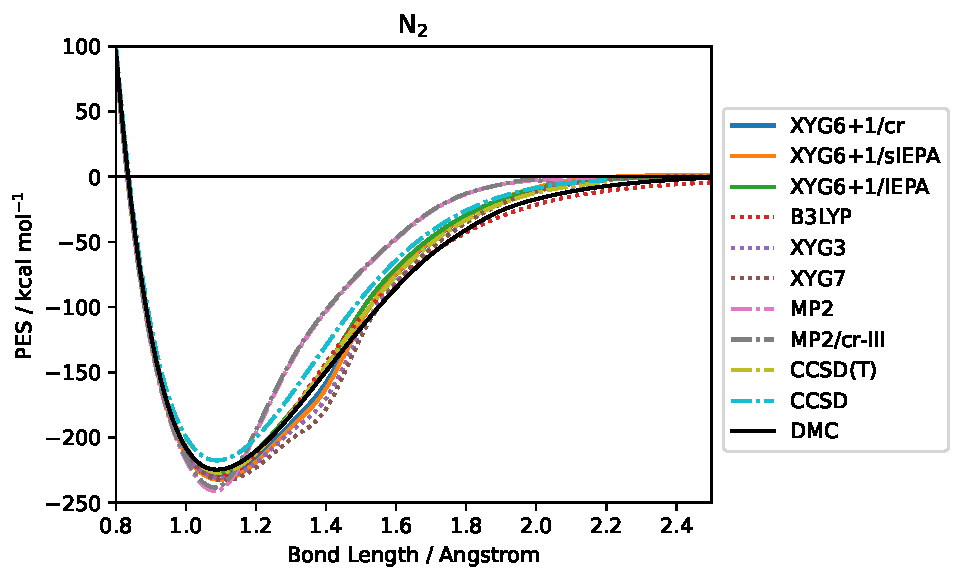
\includegraphics[width=0.7\textwidth]{assets/curve-N2-stab.pdf}
  \caption[\ce{N2} 解离曲线表现 (开壳层)]{各方法在 \ce{N2} 解离曲线的表现。参考态方法均在开壳层下优化到稳定。}
  \label{fig.2.curve-N2-stab}
\end{figure}

\begin{figure}[!h]
  \centering
  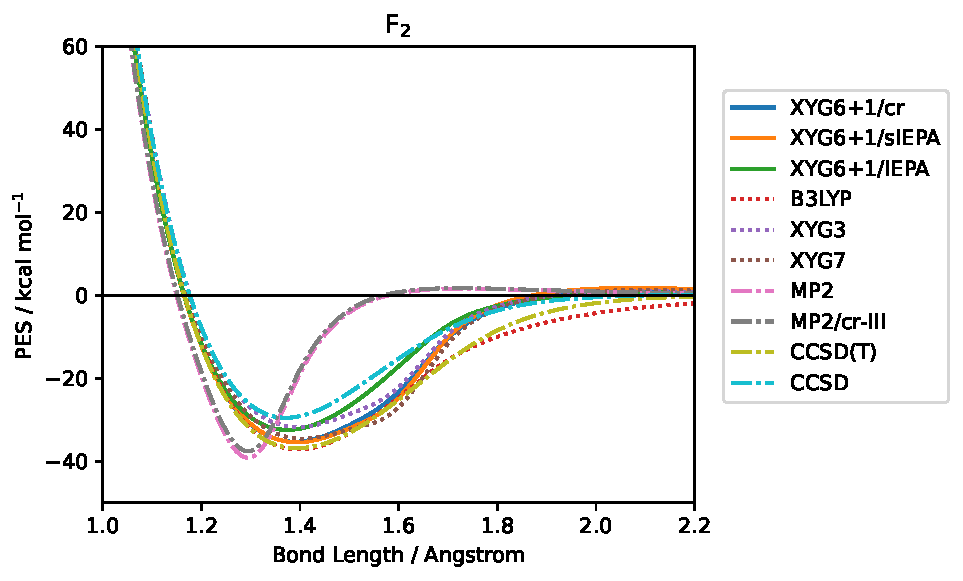
\includegraphics[width=0.7\textwidth]{assets/curve-F2-stab.pdf}
  \caption[\ce{F2} 解离曲线表现 (开壳层)]{各方法在 \ce{F2} 解离曲线的表现。参考态方法均在开壳层下优化到稳定。}
  \label{fig.2.curve-F2-stab}
\end{figure}

\begin{figure}[!h]
  \centering
  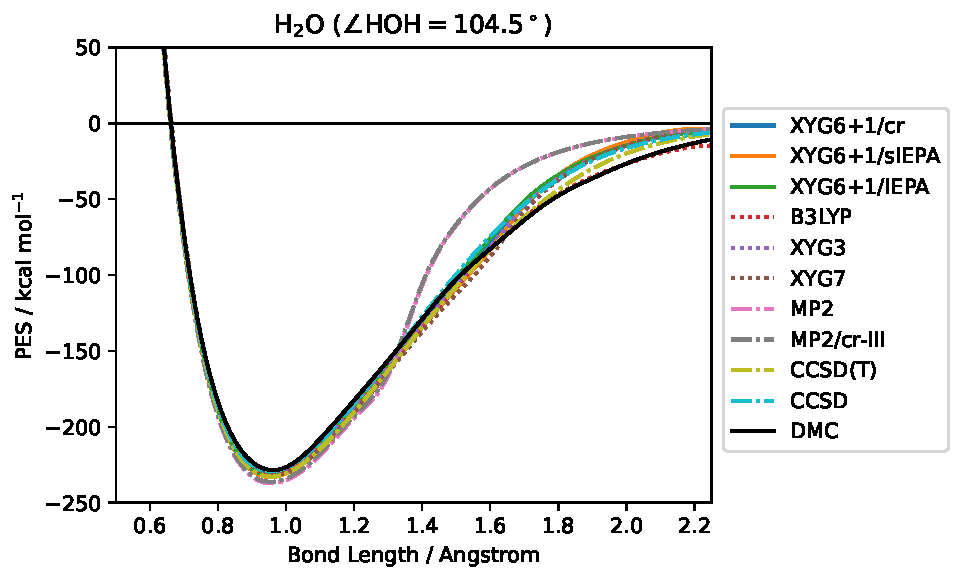
\includegraphics[width=0.7\textwidth]{assets/curve-H2O-stab.pdf}
  \caption[\ce{H2O} 解离曲线表现 (开壳层)]{各方法在 \ce{H2O} 解离曲线的表现。参考态方法均在开壳层下优化到稳定。}
  \label{fig.2.curve-H2O-stab}
\end{figure}

\begin{figure}[!h]
  \centering
  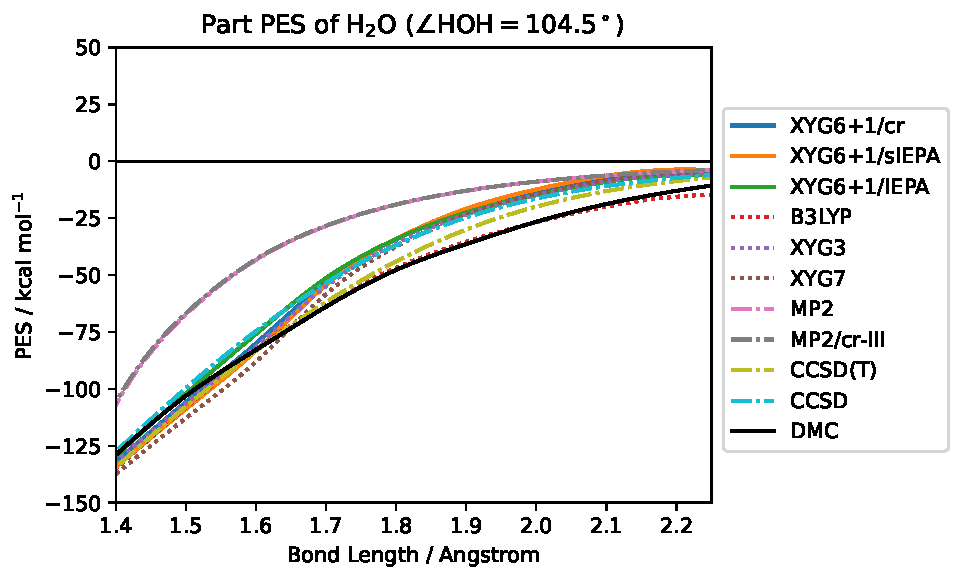
\includegraphics[width=0.7\textwidth]{assets/curve-H2O-part-stab.pdf}
  \caption[\ce{H2O} 解离曲线 1.4--2.25 \AA 段表现 (开壳层)]{各方法在 \ce{H2O} 解离曲线 1.4--2.25 \AA 段的表现。参考态方法均在开壳层下优化到稳定。}
  \label{fig.2.curve-H2O-part-stab}
\end{figure}

\begin{figure}[!h]
  \centering
  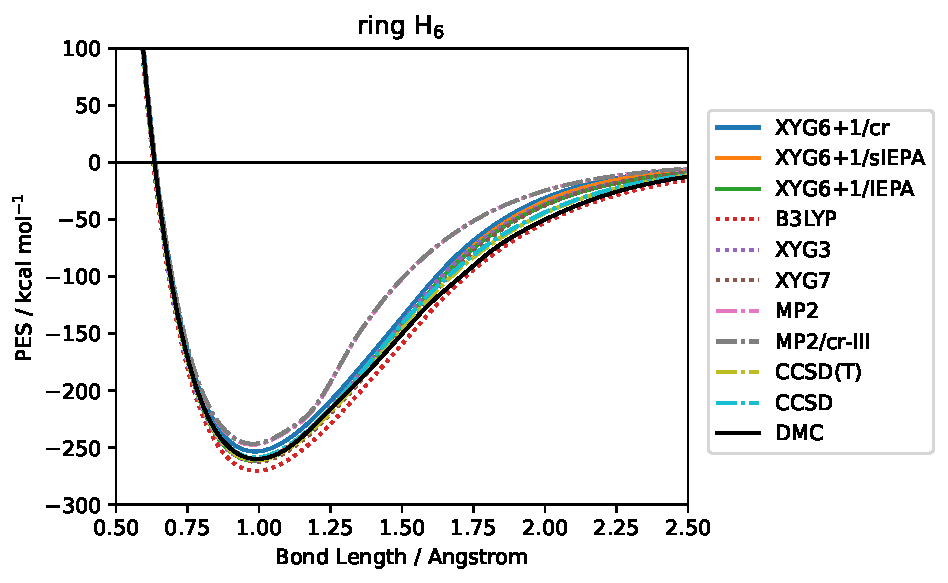
\includegraphics[width=0.7\textwidth]{assets/curve-H6-stab.pdf}
  \caption[\ce{H6} 解离曲线表现 (开壳层)]{各方法在 \ce{H6} 解离曲线的表现。参考态方法均在开壳层下优化到稳定。}
  \label{fig.2.curve-H6-stab}
\end{figure}

\subsection{电子对方法不具有正交不变性的说明}

正交变换不变性与大小可延展性,是电子结构方法非常关心的基本性质。目前流行的众多波函数方法,诸如 CCSD、MP2,以及密度泛函近似,都具有正交不变性与大小可延展性。一般来说,大小可延展性是电子结构方法推向实用过程中,必须要满足的性质。以 CID 方法为例,若不满足大小可延展性,能量便不随着体系的增大而线性地增加;这将产生相当严重的数值误差。大多数情况下,满足大小一致性的方法,其大小可延展性也可以得到满足。

从实用性角度来看,正交变换不变性相对来说重要性较低;但作为电子结构方法,它也是应当得以满足的性质。对分子轨道的正交变换,会使得 Hartree-Fock 参考态对应分子轨道基的 Fock 矩阵并非对角矩阵。与 MP2 方法不同,本工作所考虑的电子对方法 MP2/cr 与 IEPA,其定义须基于正则 Hartree-Fock 轨道。因此,从定义上,MP2/cr 与 IEPA 方法等电子对方法,无法对非正则 Hartree-Fock 作计算,故而不存在正交不变性。因而,XYG6+1 模型下的泛函近似也不具有正交不变性。

但是,对于正则 Hartree-Fock 能级简并的分子轨道,正交变换后的分子轨道仍然是正则的。此时,IEPA 或 MP2/cr 等电子对方法仍然是可以被定义的;从而,对能级简并分子轨道的正交变换不变性是可以讨论的。简并轨道可能源于下述四种情况:
\begin{enumerate}[nosep]
  \item 距离无穷远的两个完全等价体系产生的成对简并轨道;
  \item 因分子点群对称性而在二维不可约表示下产生的二重简并轨道;
  \item 因分子点群对称性而在三维不可约表示下产生的三重简并轨道;
  \item 偶然的能级简并。
\end{enumerate}
针对这些情形,我们将作简单的讨论与分析,并将表明本工作所考虑的电子对方法 (MP2/cr、IEPA) 依情况并非正交不变;同时,因简并分子轨道正交变换而导致的能量变化通常不严重,但也存在正交变换误差大于 0.5 eV 的情形。由于从表达式上,sIEPA 与 IEPA 具有相似的形式;因此,若 IEPA 并非正交不变,那么容易知道 sIEPA 也同样并非正交不变。但由于 sIEPA 引入了 erfc 形式的放缩函数,因此正交变换误差通常小于 IEPA。

IEPA 方法具有大小可延展性是广为接受的结论\cite{Szabo-Ostlund.Dover.1996}。对于上述第 1 种情形的讨论,将顺带证明 MP2/cr 方法的大小一致性,从而自然具有大小可延展性。因此,本章讨论的 XYG6+1 模型下的泛函近似具有大小可延展性。

这一小节的推演将基于自旋轨道,数值结果展现将基于闭壳层轨道。一些结论展示于表 \ref{tab.2.invariance-mp2cr-iepa}。该节的数值计算使用 cc-pVDZ 基组,程序使用 \textsc{PySCF} 与 \textsc{dh}。

\begin{table}[ht]
\centering
\caption[MP2/cr 与 IEPA 在不同情形下的正交变换不变性]{MP2/cr 与 IEPA 在不同情形下能级简并轨道间的正交变换不变性。}
\label{tab.2.invariance-mp2cr-iepa}
\widetabular{
  \begin{tabular}{cccl}
  \toprule
  情形 & MP2/cr & IEPA & 情形描述   \\
  \midrule
  1  & 满足 & 不满足 & 无穷远两分子 \\
  2  & 满足 & 满足 & 二维不可约  \\
  3  & 满足 & 不满足 & 三维不可约  \\
  4  & 不满足 & 不满足 & 偶然简并  \\
  \bottomrule
  \end{tabular}
}{}
\end{table}

\subsubsection{MP2/cr 方法在完全分离体系下的正交变换不变性}

对于完全分离体系,即距离无穷远的分子 $A$ 与分子 $B$ 的复合物 $AB$,严格的复合物电子对方法相关能 $E_\textmt{c} (AB)$ 等于两个单体分子的能量之和 $E_\textmt{c} (A) + E_\textmt{c} (B)$。该性质在本工作中称为大小一致性。特别地,若 $A$ 与 $B$ 体系完全等价,那么就会因为完全分离的体系而产生成对的简并轨道,这些简并轨道的能量与单体 $A$ 或 $B$ 的轨道能量一致;在这些简并轨道的正交变换下,电子对相关能应当是不变的。

作为近似的相关能计算方法,对于这类完全分离体系问题,在 M{\o}ller-Plesset 微扰收敛的前提下,MP2 是大小一致且正交变换不变的\cite{Szabo-Ostlund.Dover.1996, Shavitt-Bartlett.Cambridge.2009};而 IEPA 方法依占据轨道的选取并非正交不变 (因此不是严格的大小一致),但仍然是大小可延展的\cite{Szabo-Ostlund.Dover.1996, Zhang-Scheffler.NJP.2016},即随着分离体系中的独立子体系的增多、相关能大致线性地增加。

这一小节将表明,对于 $A$ 与 $B$ 完全等价的情形,在特定的局域基下,它们构成的完全分离体系的复合物 $AB$ 的 MP2/cr 方法相关能 $E_\textmt{c}^\textmt{MP2/cr} (AB)$ 确实等于单体相关能之和 $E_\textmt{c}^\textmt{MP2/cr} (A) + E_\textmt{c}^\textmt{MP2/cr} (B)$。同时,在假定 $A, B$ 分子各自没有简并的占据轨道情形下,复合物 $AB$ 的一对占据简并轨道正交变换下能量不变。

\paragraph{MP2/cr 方法因完全分离体系而简并的轨道下正交不变性}

令 $i, j, \cdots$ 与 $a, b, \cdots$ 为\textbf{单体} $A$ 或 $B$ 的占据与未占轨道。使用下角标 $A$ 与 $B$ 以区分轨道所在的分离单体。对于复合物 $AB$,若其分子轨道基选取为 $i_A, j_A, \cdots, \allowbreak a_A, b_A, \allowbreak i_B, j_B, \cdots, \allowbreak a_B, b_B$,则称其为\textbf{局域基}。由于 $A$ 与 $B$ 完全分离,因此局域基是 Hartree-Fock 的正则轨道。

为简化记号表述,这里省去成对电子能量 $e_{ij}^\textmt{MP2/cr}$ 与相关能 $E_\textmt{c}^\textmt{MP2/cr}$ 的上标 $\textmt{MP2/cr}$。

对于分子 $A$ 上的占据轨道 $l_A$ 与分子 $B$ 上的占据轨道 $l_B$,定义正交变换后的分子轨道 $\mathscr{l}_1$ 与 $\mathscr{l}_2$ 为
\begin{align}
  \label{eq.2.invariance-general}
  \begin{aligned}
    \mathscr{l}_1 &= \cos(\theta) l_A - \sin(\theta) l_B \\
    \mathscr{l}_2 &= \sin(\theta) l_A + \cos(\theta) l_B
  \end{aligned}
\end{align}
我们称 $\theta$ 为正交变换相位。特别地,在该段落中,我们仅对 $\theta = - \pi/4$ 的情形作讨论:
\begin{align}
  \label{eq.2.invariance-specific}
  \mathscr{l}_1 = \frac{1}{\sqrt{2}} (l_A + l_B), \quad \mathscr{l}_2 = \frac{1}{\sqrt{2}} (l_A - l_B)
\end{align}
除了 $l_A$ 与 $l_B$ 轨道作正交变换外,其余轨道均与局域基相同。这里称其为\textbf{离域基}。

首先简要表明 MP2/cr 方法在局域基下是大小一致的。简记分子轨道基的 ERI 张量 $\langle ij | ab \rangle$ 为 $g_{ij}^{ab}$,则对于分离的单体而言,对应式 (\ref{eq.2.eij-MP2cr}),成对电子 $ij$ 的相关能为
\begin{equation*}
  e_{ij} = \frac{1}{2} \sum_{ab} \frac{1}{N_{ij}} \frac{\big( g_{ij}^{ab} - g_{ij}^{ba} \big)^2}{D_{ij}^{ab}} = \frac{1}{2} \sum_{ab} \frac{1}{N_{ij}} \big( t_{ij}^{ab} \big)^2 D_{ij}^{ab}
\end{equation*}
MP2 激发张量 $t_{ij}^{ab}$ 是
\begin{equation*}
  t_{ij}^{ab} = \frac{g_{ij}^{ab} - g_{ij}^{ba}}{D_{ij}^{ab}}
\end{equation*}
MP2/cr 缩放比例 $N_{ij}$ 定义式在 (\ref{eq.2.Nij-MP2cr}) 已有表述。

对于复合物 $AB$ 的局域基,首先注意到 ERI 张量中,若有轨道分属于不同的原子,那么该张量元的值为零;即仅有类似于 $g_{i_A j_A}^{a_A b_A}$ 或 $g_{i_B j_B}^{a_B b_B}$ 的元素非零。可以得知的推论是,MP2 激发张量也仅有类似于 $t_{i_A j_A}^{a_A b_A}$ 或 $t_{i_B j_B}^{a_B b_B}$ 的元素非零;进而
\begin{gather*}
  N_{i_A j_A} = N_{i_B j_B} = N_{ij}, \quad N_{i_A j_B} = N_{i_A j_B} = 0 \quad (\forall i, j) \\
  e_{i_A j_A} = e_{i_B j_B} = e_{ij}, \quad e_{i_A j_B} = e_{i_A j_B} = 0 \quad (\forall i, j) \\
  E_\textmt{c} (AB) = \frac{1}{2} \sum_{i_A j_A} e_{i_A j_A} + \frac{1}{2} \sum_{i_B j_B} e_{i_B j_B} = \sum_{ij} e_{ij} = E_\textmt{c} (A) + E_\textmt{c} (B) \quad \text{(localized basis)}
\end{gather*}
因此容易表明,MP2/cr 在局域基下是大小一致的。

随后需要说明 MP2/cr 在离域基下的相关能与局域基是相同的。首先,$l_A$ 与 $l_B$ 的轨道能均为 $\varepsilon_l$;因此,对这两根轨道正交变换后,得到的 $\mathscr{l}_1$ 与 $\mathscr{l}_2$ 轨道能仍然有
\begin{equation*}
  \varepsilon_{\mathscr{l}_1} = \varepsilon_{\mathscr{l}_2} = \varepsilon_l
\end{equation*}
对于离域基,显然地,占据轨道中并非 $\mathscr{l}_1$ 与 $\mathscr{l}_2$ 的部分,其结果与局域基完全一致。因此,我们仅讨论涉及 $\mathscr{l}_1$ 与 $\mathscr{l}_2$ 的部分。对于 ${i_A \mathscr{l}_1}$ 电子对的情形 ($\forall i \neq l$),注意到对于 $\forall a, b$,
\begin{align*}
  g_{i_A \mathscr{l}_1}^{a_A b_A} &= \frac{1}{\sqrt{2}} g_{i_A l_A}^{a_A b_A} + \frac{1}{\sqrt{2}} g_{i_A l_B}^{a_A b_A} = \frac{1}{\sqrt{2}} g_{il}^{ab} \\
  t_{i_A \mathscr{l}_1}^{a_A b_A} &= \frac{1}{\sqrt{2}} \frac{g_{i_A l_A}^{a_A b_A} - g_{i_A l_A}^{b_A a_A}}{D_{il}^{ab}} = \frac{1}{\sqrt{2}} t_{il}^{ab}
\end{align*}
对于 $g_{i_A \mathscr{l}_2}^{a_A b_A}$ 与 $t_{i_A \mathscr{l}_2}^{a_A b_A}$ 有同样的结论。对于 $\mathscr{l}_1 \mathscr{l}_2$ 电子对的情形,注意到 ERI 张量的对称性 $g_{l_A l_A}^{a_A b_A} = g_{l_A l_A}^{b_A a_A}$,因此
\begin{align*}
  g_{\mathscr{l}_1 \mathscr{l}_2}^{a_A b_A} &= \frac{1}{2} g_{l_A l_A}^{a_A b_A} \\
  t_{\mathscr{l}_1 \mathscr{l}_2}^{a_A b_A} &= \frac{1}{2} \frac{g_{l_A l_A}^{a_A b_A} - g_{l_A l_A}^{b_A a_A}}{D_{il}^{ab}} = 0
\end{align*}
对于分子 $B$ 的情况也是类似的:
\begin{gather*}
  t_{i_B \mathscr{l}_1}^{a_B b_B} = - t_{i_B \mathscr{l}_2}^{a_B b_B} = \frac{1}{\sqrt{2}} t_{ij}^{ab} , \quad
  t_{\mathscr{l}_1 \mathscr{l}_2}^{a_B b_B} = 0
\end{gather*}

因此,对于 $\forall i, j \neq l$,
\begin{align*}
  N_{i_A j_A} &= 1 + \frac{1}{2} \sum_{\substack{k_A \neq l_A \\ a_A b_A}} \left( \big( t_{i_A k_A}^{a_A b_A} \big)^2 + \big( t_{j_A k_A}^{a_A b_A} \big)^2 \right) \\
  &\quad + \frac{1}{2} \left( \big( t_{i_A \mathscr{l}_1}^{a_A b_A} \big)^2 + \big( t_{i_A \mathscr{l}_2}^{a_A b_A} \big)^2 + \big( t_{j_A \mathscr{l}_1}^{a_A b_A} \big)^2 + \big( t_{j_A \mathscr{l}_2}^{a_A b_A} \big)^2 \right) \\
  &= 1 + \frac{1}{2} \sum_{\substack{k \neq l \\ ab}} \left( \big( t_{ik}^{ab} \big)^2 + \big( t_{jk}^{ab} \big)^2 \right) \\
  &\quad + \frac{1}{2} \left( \frac{1}{2} \big( t_{il}^{ab} \big)^2 + \frac{1}{2} \big( t_{il}^{ab} \big)^2 + \frac{1}{2} \big( t_{jl}^{ab} \big)^2 + \frac{1}{2} \big( t_{jl}^{ab} \big)^2 \right) \\
  &= 1 + \frac{1}{2} \sum_{kab} \left( \big( t_{ik}^{ab} \big)^2 + \big( t_{jk}^{ab} \big)^2 \right) \quad \text{(delocalized basis)}
\end{align*}
即对于 $\forall i, j \neq l$,缩放系数 $N_{i_A j_A}$ 不论是局域基还是离域基下,结果均相同。因此,可以证明成对电子 $i_A j_A$ 相关能也是一致的:
\begin{equation*}
  e_{i_A j_A} = \frac{1}{2} \sum_{ab} \frac{1}{N_{i_A j_A}} \big( t_{i_A j_A}^{a_A b_A} \big)^2 D_{ij}^{ab} = \frac{1}{2} \sum_{ab} \frac{1}{N_{ij}} \big( t_{ij}^{ab} \big)^2 D_{ij}^{ab} = e_{ij} \quad \text{(delocalized basis)}
\end{equation*}
上述结论对于分子 $B$ 同理。

对于 $\forall i \neq l$,首先注意到 MP2 激发张量中,相同占据轨道的元素是零,举例而言即 $t_{i_A i_A}^{a_A b_A} = 0$ 或 $t_{\mathscr{l}_1 \mathscr{l}_1}^{a_A b_A} = 0$ ($\forall i, a, b$);但同时需要注意到,回顾式 (\ref{eq.2.Nij-MP2cr}),对于 $AB$ 复合物而言,被求和的指标包括 $A$ 分子与 $B$ 分子的所有轨道,因此
\begingroup
\allowdisplaybreaks
\begin{align*}
  N_{i_A \mathscr{l}_1} &= 1 + \frac{1}{2} \sum_{\substack{k_A \neq l_A \\ a_A b_A}} \big( t_{i_A k_A}^{a_A b_A} \big)^2 + \frac{1}{2} \big( t_{i_A \mathscr{l}_1}^{a_A b_A} \big)^2 + \frac{1}{2} \big( t_{i_A \mathscr{l}_2}^{a_A b_A} \big)^2 \\
  &\quad + \frac{1}{2} \sum_{\substack{k_A \neq l_A \\ a_A b_A}} \big( t_{\mathscr{l}_1 k_A}^{a_A b_A} \big)^2 + \frac{1}{2} \sum_{\substack{k_B \neq l_B \\ a_B b_B}} \big( t_{\mathscr{l}_1 k_B}^{a_B b_B} \big)^2 + \frac{1}{2} \big( t_{\mathscr{l}_1 \mathscr{l}_1}^{a_A b_A} \big)^2 + \frac{1}{2} \big( t_{\mathscr{l}_1 \mathscr{l}_2}^{a_A b_A} \big)^2 \\
  &= 1 + \frac{1}{2} \sum_{\substack{k \neq l \\ ab}} \big( t_{ik}^{ab} \big)^2 + \frac{1}{4} \big( t_{il}^{ab} \big)^2 + \frac{1}{4} \big( t_{il}^{ab} \big)^2 \\
  &\quad + \frac{1}{4} \sum_{\substack{k \neq l \\ ab}} \big( t_{lk}^{ab} \big)^2 + \frac{1}{4} \sum_{\substack{k \neq l \\ ab}} \big( t_{lk}^{ab} \big)^2 + 0 + 0 \\
  &= 1 + \frac{1}{2} \sum_{kab} \left( \big( t_{ik}^{ab} \big)^2 + \big( t_{lk}^{ab} \big)^2 \right) \quad \text{(delocalized basis)}
\end{align*}
\endgroup
因此,对于 $\forall i \neq l$,缩放系数离域基下的 $N_{i_A \mathscr{l}_1}$ 与局域基下的 $N_{i_A l_A}$ 的结果、或者 $A$ 或 $B$ 单体的 $N_{ij}$ 相等。因此,
\begin{equation*}
  e_{i_A \mathscr{l}_1} = \sum_{a_A b_A} \frac{1}{N_{i_A \mathscr{l}_1}} \big( t_{i_A \mathscr{l}_1}^{a_A b_A} \big)^2 D_{il}^{ab} = \frac{1}{2} \sum_{ab} \frac{1}{N_{il}} \big( t_{il}^{ab} \big)^2 D_{il}^{ab} = \frac{1}{2} e_{il} \quad \text{(delocalized basis)}
\end{equation*}
从而,离域基下的成对电子能 $e_{i_A \mathscr{l}_1}$ 是单个分子的 $e_{il}$ 的一半。类似地可以表明,离域基下,
\begin{equation*}
  e_{i_A \mathscr{l}_2} = e_{i_B \mathscr{l}_1} = e_{i_B \mathscr{l}_2} = \frac{1}{2} e_{il} \quad \text{(delocalized basis)}
\end{equation*}

对于离域基下的占据电子对 $\mathscr{l}_1 \mathscr{l}_2$,注意到先前已表明 $t_{\mathscr{l}_1 \mathscr{l}_2}^{a_B b_B} = 0$ ($\forall a, b$),因此容易知道 $e_{\mathscr{l}_1 \mathscr{l}_2} = 0$。

因此,可以推知离域基下,复合物 $AB$ 的 MP2/cr 相关能为
\begin{align*}
  E_\textmt{c} (AB) &= \frac{1}{2} \sum_{i_A j_A \neq l_A} e_{i_A j_A} + \sum_{i_A \neq l_A} \big( e_{i_A \mathscr{l}_1} + e_{i_A \mathscr{l}_2} \big) \\
  &\quad + \frac{1}{2} \sum_{i_B j_B \neq l_B} e_{i_B j_B} + \sum_{i_B \neq l_B} \big( e_{i_B \mathscr{l}_1} + e_{i_B \mathscr{l}_2} \big) + e_{\mathscr{l}_1 \mathscr{l}_2} \\
  &= \frac{1}{2} \sum_{ij \neq l} e_{ij} + \sum_{i \neq l} e_{il} \\
  &\quad + \frac{1}{2} \sum_{ij \neq l} e_{ij} + \sum_{i \neq l} e_{il} + 0 \\
  &= \sum_{ij} e_{ij} = E_\textmt{c} (A) + E_\textmt{c} (B) \quad \text{(delocalized basis)}
\end{align*}
该离域基下的复合物 $AB$ 相关能与 $A$、$B$ 单体的相关能之和完全相等。

上述讨论表明,尽管离域基与局域基并不等同;但复合物 $AB$ 的能量,在相同能级轨道的式 (\ref{eq.2.invariance-specific}) 定义下的正交变换下是不变的。

尽管我们仅仅针对式 (\ref{eq.2.invariance-specific}) 的特殊情况,作正交不变性的说明;但可以预期,若针对因等同分离体系而简并的占据或非占轨道,作式 (\ref{eq.2.invariance-general}) 下各种角度 $\theta$ 的正交变换,相关能 $E_\textmt{c} (AB)$ 仍然不变。

\paragraph{接近完全分离体系的正交变换误差数值表现}

与式 (\ref{eq.2.invariance-general}) 相同地,对于两个独立体系 $A$ 与 $B$,构造轨道 $\mathscr{i}_1, \mathscr{i}_2$ 为分子轨道 $i_A, i_B$ 的线性组合
\begin{align*}
  \mathscr{i}_1 &= \cos(\theta) i_A - \sin(\theta) i_B \\
  \mathscr{i}_2 &= \sin(\theta) i_A + \cos(\theta) i_B
\end{align*}
当正交变换相位 $\theta$ 变换到 $\pi/2$ 时,则恰好交换了 $i_A$ 与 $i_B$;因此我们仅需要考察 $\theta \in [0, \pi/2]$ 的区间。由于 MP2 容易被证明、MP2/cr 已经由上文说明在当前的正交变换下是不变的,因此可以预期这两种方法的正交变换误差严格为零。

\begin{figure}[!ht]
  \centering
  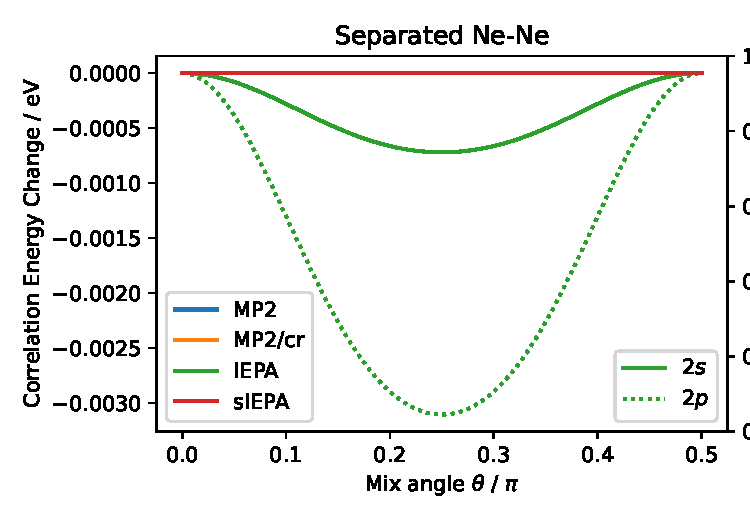
\includegraphics[width=0.6\textwidth]{assets/invar-sep-Ne.pdf}
  \caption[\ce{Ne2} 对称性简并轨道正交变换误差]{距离 100 \AA 的 \ce{Ne2} 的相关能随正交变换相位 $\theta$ 变化产生的误差。右下角图例表示被正交变换对应的单体分子轨道。该情形下 MP2、MP2/cr、sIEPA 的误差均为零或极其接近零,图上的曲线重合。}
  \label{fig.2.invar-sep-Ne}
\end{figure}

对于原子之间距离 100 \AA 的 \ce{Ne2} 体系,成对电子型相关能 $E_\textmt{c}^\textmt{EP}$ 依正交变换相位 $\theta$ 的变化情况展示于图 \ref{fig.2.invar-sep-Ne}。对于该体系,100 \AA 的距离可以看作相互没有影响 (复合物 MP2 相关能相比于两个 \ce{Ne} 原子相关能之和的误差是 \num{6e-8} eV,接近于自洽场能量收敛限)。对于该复合物的轨道正交变换,其导致的能量误差不超过 0.005 eV 或 0.1 kcal/mol;这种程度的影响并不是很大。作为比较,CISD 方法尽管是正交不变、但却是大小不可延展的;对于当前体系,距离 100 \AA 的 \ce{Ne2} 体系相关能与两个单独的 \ce{Ne} 原子相关能相差 0.246 eV。

注意到 sIEPA 在两个 \ce{Ne} 原子体系下接近于正交变换不变。这是因为 sIEPA 在 HOMO/LUMO gap 较大的情形下迅速退化到 MP2 (对于当前体系,sIEPA 与 MP2 能量的误差在机器精度即 $2^{-53}$ Hartree 量级)。因此,尽管 sIEPA 与 IEPA 有相似的表达形式、显然不是正交变换不变的,但其误差在 HOMO/LUMO gap 较大时,sIEPA 的正交变换误差会远小于 IEPA。

\begin{figure}[!ht]
  \centering
  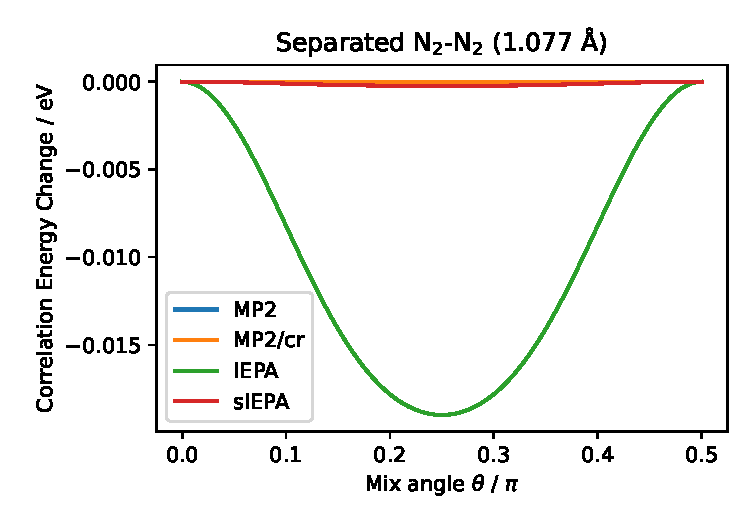
\includegraphics[width=0.6\textwidth]{assets/invar-sep-N2-1.pdf}
  \caption[\ce{N2} 对称性简并轨道正交变换误差 (键长 1.077 \AA)]{距离 100 \AA 的 \ce{N2} 的相关能随正交变换相位 $\theta$ 变化产生的误差。\ce{N2} 键长为 HF/cc-pVDZ 下平衡键长 1.077 \AA。右下角图例表示被正交变换对应的单体分子轨道。该情形下 MP2、MP2/cr、sIEPA 的误差均为零或极其接近零,图上的曲线重合。}
  \label{fig.2.invar-sep-N2-1}
\end{figure}

\begin{figure}[!ht]
  \centering
  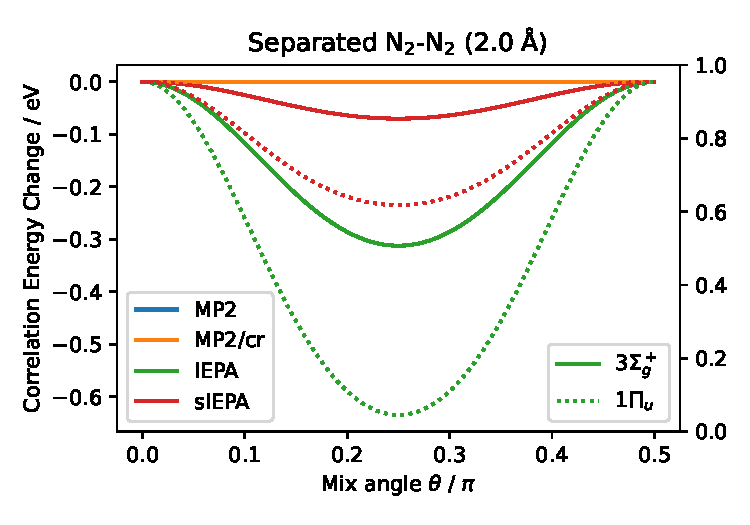
\includegraphics[width=0.6\textwidth]{assets/invar-sep-N2-2.pdf}
  \caption[\ce{N2} 对称性简并轨道正交变换误差 (键长 2.0 \AA)]{距离 100 \AA 的 \ce{N2} 的相关能随正交变换相位 $\theta$ 变化产生的误差。\ce{N2} 键长为 2.0 \AA。右下角图例表示被正交变换对应的单体分子轨道。该情形下 MP2、MP2/cr 的误差均为零,图上的曲线重合。}
  \label{fig.2.invar-sep-N2-2}
\end{figure}

如 Szabo 与 Ostlund 在 5.1.1 小节中对模型体系的讨论\cite{Szabo-Ostlund.Dover.1996},影响 IEPA 方法的正交变换误差,受轨道能量差与双电子积分的共同影响。其中,轨道能差的影响较为关键;被变换轨道与分子的 HOMO 或 LUMO 越接近,正交变换的误差就越大。对于两个 \ce{Ne} 原子体系而言,$2p$ 轨道的能级相比于 $2s$ 更高、与 LUMO 能级更接近,因此有更大的正交变换误差。从图 \ref{fig.2.invar-sep-N2-1} 与图 \ref{fig.2.invar-sep-N2-2} 上可以看出,对于两个 \ce{N2} 原子体系,若对其 HOMO 轨道 ($1 \symup{\Pi}_u$) 作正交变换,该情形更为明显。当 \ce{N2} 键长较短时,IEPA 的正交变换误差是较小的 $-0.019$ eV;但当 \ce{N2} 键长较长时,IEPA 的正交变换误差是较大的 $-0.635$ eV。同时,键长较长时,由于 HOMO/LUMO gap 较小,因此 sIEPA 不再与 MP2 有相似的数值,从而 sIEPA 显现出较大的正交变换误差。

\subsubsection{因点群对称性而简并的轨道下正交不变性}

\paragraph{MP2/cr 该情形下正交不变性的简要说明}

MP2/cr 方法在数值计算结果上,对于因点群对称性而简并的轨道,显现出正交不变性。这里对 MP2/cr 方法在该情形下的正交不变性作不严格的说明。

首先,定义其中一种分子轨道基为 $i, j, \cdots, a, b, \cdots$。当前我们仅考虑占据轨道上的实正交变换;变换后的基为 $i', j', \cdots, a, b, \cdots$;变换后的张量上标波浪号。占据轨道的正交变换矩阵记为 $U_{i' i}$;若变换前的分子轨道到原子轨道线性组合的系数矩阵是 $C_{\mu i}$,则变换后的系数矩阵 $\tilde{C}_{\mu i'}$ 是
\begin{equation*}
  \tilde{C}_{\mu i'} = \sum_{i} C_{\mu i} U_{i' i}
  \quad \text{or} \quad
  \tilde{\mathbf{C}} = \mathbf{C} \mathbf{U}^\dagger
\end{equation*}
由于我们仅考虑因点群对称性而简并的轨道,因此 $U_{i' i}$ 矩阵除了简并轨道外,其余部分是单位矩阵。由于 ERI 张量对轨道的变换是线性的,因此容易表明对于下述定义的矩阵 $\mathscr{G}_{ij}$
\begin{equation*}
  \mathscr{G}_{ij} = \sum_{kab} g_{ik}^{ab} g_{jk}^{ab}
\end{equation*}
轨道变换后的矩阵有
\begin{equation*}
  \tilde{\mathscr{G}}_{i'j'} = \sum_{ij} U_{i' i} \mathscr{G}_{ij} U_{j' j}
  \quad \text{or} \quad
  \tilde{\symbfscr{G}} = \mathbf{U} \symbfscr{G} \mathbf{U}^\dagger
\end{equation*}
由于轨道变换不影响能级,因此对于下述定义的矩阵 $\mathscr{T}_{ij}$
\begin{equation*}
  \mathscr{T}_{ij} = \sum_{kab} t_{ik}^{ab} t_{jk}^{ab}
\end{equation*}
同样容易验证有
\begin{equation*}
  \tilde{\mathscr{T}}_{i'j'} = \sum_{ij} U_{i' i} \mathscr{T}_{ij} U_{j' j}
  \quad \text{or} \quad
  \tilde{\symbfscr{T}} = \mathbf{U} \symbfscr{T} \mathbf{U}^\dagger
\end{equation*}

回顾到 MP2/cr 的定义,式 (\ref{eq.2.Nij-MP2cr}) 所给出的缩放系数 $N_{ij}$ 同样可以写为
\begin{equation*}
  N_{ij} = 1 + \frac{1}{2} \big( \mathscr{T}_{ii} + \mathscr{T}_{jj} \big)
\end{equation*}
因此,尽管缩放系数的指标是成对电子 $ij$,但实际上仅由单指标的对角元 $\mathscr{T}_{ii}$ 确定。注意到我们变换的是二维或三维不可约表示下简并轨道;这些轨道之间在对称性上相互正交,因此 $\symbfscr{T}$ 矩阵在被变换的轨道上非对角元为零。同时,这些简并轨道出于相同的对称性,矩阵 $\symbfscr{T}$ 在这些简并轨道上的对角元数值相等,即是单位矩阵的倍数。在正交变换下,单位矩阵不变;因此,变换后的矩阵对角元 $\tilde{\mathscr{T}}_{i'i'}$ 对于被变换的简并轨道并未改变。对于没有被变换的轨道,正交变换矩阵 $U_{i'i}$ 在这些轨道上是单位矩阵,因此变换后的 $\tilde{\mathscr{T}}_{i' j'}$ 与变换前的 $\mathscr{T}_{ij}$ 相同。从而,正交变换后的 $\tilde{N}_{i'j'}$ 与变换前的 $N_{ij}$ 完全相同。

这里不对总相关能 $E_\textmt{c}^\textmt{MP2/cr}$ 的正交不变性作证明,但作补充说明与推测。成对电子能量 $e_{ij}^\textmt{MP2/cr}$ 在上述正交变换下,\textbf{并非}与 $\tilde{e}_{i'j'}^\textmt{MP2/cr}$ 相等;但对于 $i$ 代表被正交变换的基、$j$ 代表能级相同但未被正交变换的另一组基,那么对这些特定占据轨道的 $\sum_{ij} e_{ij}^\textmt{MP2/cr}$ 正交变换前后是不变的。从而,总相关能 $E_\textmt{c}^\textmt{MP2/cr}$ 在当前的正交变换下,也是不变的。

\paragraph{点群对称性下简并轨道正交变换误差数值表现}

数值计算的体系选用 \ce{C4H4} 模型体系;该体系为 $T_d$ 点群,碳原子之间构成正四面体且键长为 2 \AA;氢原子与临近碳原子的键长为 2 \AA。该体系的电子共 14 对,占据排布是
$$
(1 A_1)^2 (1 T_2)^6 (2 A_1)^2 (2 T_2)^6 (3 A_1)^2 (3 T_2)^6 (1 E)^4
$$
我们分别考察 $3 T_d$ 和 $1 E$ 内部的电子正交变换。对于 $1E$ 的占据轨道,对其正交变换的方式在式 (\ref{eq.2.invariance-general}) 中定义;对于 $3 T_d$ 的占据轨道,我们仅旋转其中的两组,旋转过程也与式 (\ref{eq.2.invariance-general}) 一致。

\begin{figure}[!ht]
  \centering
  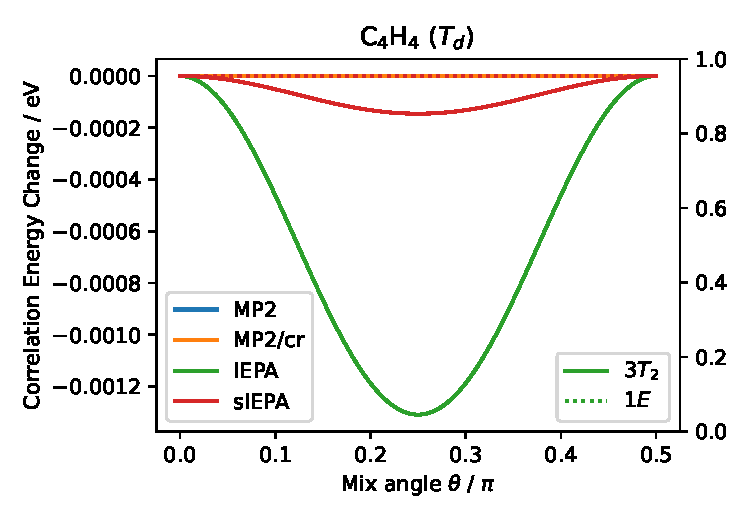
\includegraphics[width=0.6\textwidth]{assets/invar-sep-C4H4-1.pdf}
  \caption[$T_d$ 点群下 \ce{C4H4} 对称性简并轨道正交变换误差]{$T_d$ 点群下 \ce{C4H4} 的相关能随相同不可约表示简并轨道下正交变换相位 $\theta$ 变化产生的误差。右下角图例表示被正交变换对应的分子轨道。该情形下 MP2、MP2/cr 的误差,以及 $1E$ 轨道下所有方法的误差均为零,图上的曲线重合。}
  \label{fig.2.invar-sep-C4H4-1}
\end{figure}

对于当前情形,正交变换的相关能误差展示于图 \ref{fig.2.invar-sep-C4H4-1}。可以看到,对于二维不可约表示 $E$,所有方法都表现出了正交变换的不变性。但对于 $T_2$ 不可约表示,IEPA 与 sIEPA 方法存在一定的正交变换误差;其中,IEPA 方法误差最大为 $-0.0013$ eV,对于当前体系是相当小的数值。

\subsubsection{偶然能级简并的正交不变性}

这里仅使用数值表现,表明 MP2/cr 与 IEPA 均在偶然能级简并的轨道正交变换下存在误差。这里考察键长为 1.82116696109 \AA 的 \ce{CO} 分子。该分子的占据排布是
$$
(1 \symup{\Sigma}^+)^2 (2 \symup{\Sigma}^+)^2 (3 \symup{\Sigma}^+)^2 (4 \symup{\Sigma}^+)^2 (1 \symup{\Pi})^4 (5 \symup{\Sigma}^+)^2
$$
RHF/cc-pVDZ 基组下以能量 \num{1e-13} Hartree、轨道梯度 \num{1e-11} Hartree 为收敛限时,$1 \symup{\Pi}$ 轨道与 $5 \symup{\Sigma}^+$ 轨道的能级差小于 \num{1e-11} Hartree;在当前的分析中,该能极差可以认为接近于零,即这两种轨道是简并的。我们对其中一根 $1 \symup{\Pi}$ 轨道与 $5 \symup{\Sigma}^+$ 轨道作正交变换,变换相位在式 (\ref{eq.2.invariance-general}) 中定义。对于该情形,MP2/cr 与 IEPA 方法都展现出一定的正交变换误差,但误差数值不大于 0.005 eV。尽管在完全分离体系、以及二维或三维不可约简并轨道正交变换下,MP2/cr 展现出正交不变性;但该例子可以表明,MP2/cr 一般而言不具有正交不变性。

\begin{figure}[!ht]
  \centering
  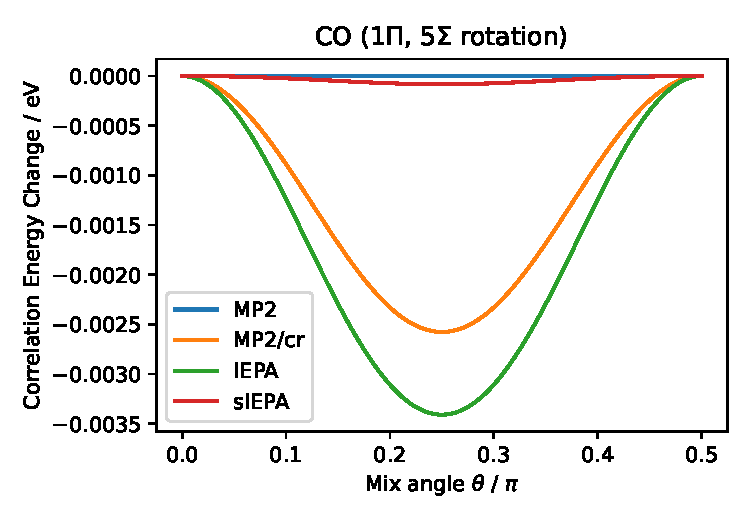
\includegraphics[width=0.6\textwidth]{assets/invar-sep-CO.pdf}
  \caption[\ce{CO} 偶然简并轨道正交变换误差]{\ce{CO} 分子的相关能在能级偶然简并的 $1 \symup{\Pi}$ 轨道与 $5 \symup{\Sigma}^+$ 轨道间依正交变换相位 $\theta$ 变化产生的误差。该情形下 MP2 的误差为零。}
  \label{fig.2.invar-sep-CO}
\end{figure}
